\section{Die Genauigkeitsmessung des Extraktionsalgorithmus}
\label{sec:evaluierung}

Der entwickelte Algorithmus deckt die grundlegenden Elementtypen für die Datenextraktion ab und ist in der Lage bis
zu 70 Seiten pro Sekunde zu verarbeiten.
Wie bereits eingangs erwähnt wurde, ist die Qualität der Extraktion von großer Bedeutung - doch wie genau ist der
entwickelte Algorithmus?
Genau diese Frage wird in diesem Kapitel beantwortet, um eine grobe Aussage für das weitere Matchingverfahren zu
treffen.

\subsection{Die Testdaten der Evaluierung}
\label{subsec:testdaten}
Sowohl für das Antrainieren der Extraktionsregeln als auch für die Evaluierung der Ergebnisse wurden die von idealo
zur Verfügung gestellten Angebotsdaten verwendet.
Für die nachfolgenden Messungen wurden 7500 Angebote von 50 Shops genutzt.

Je Händler wurden max.\ 50 Angebote als Trainingsmenge für die Erstellung der Regeln und 100 Angebote als Testmenge für
die Evaluierung verwendet.
Die Auswahl der Shops erfolgte basierend auf den ersten Listeneinträgen der Shopübersicht\footnotemark von idealo.
\footnotetext{https://www.idealo.de/preisvergleich/AllePartner.html}

Alle nachfolgenden Messungen basieren auf einem Schnappschuss der Angebotsdaten inklusive der verlinkten Webseiten.
Die Links wurden nicht durch die URL-Cleaner-Komponente bereinigt, da sonst die Angebotsdaten von idealo
möglicherweise nicht mit denen von der Webseite übereinstimmen.
Damit die Trackingstatistiken der Shopbetreiber nicht verfälscht werden, wurden nicht mehr als 150 Angebote je Shop
heruntergeladen.

Eine Analyse der gesamten Testdaten hat ergeben, dass für jedes Angebot die Angaben zum Titel, dem Preis und der SKU
existieren.
Am seltensten existieren hingegen die HAN (68\%) und die Produktbeschreibung (77\%) eines Angebots.

Das Verhältnis der fehlenden zu den vorhandenen Produktattributen der Trainingsmenge ähnelt dem Verhältnis der
Testmenge und weicht um maximal 0.88\% bei der Produkteigenschaft "Marke" ab.

\subsection{Die Messergebnisse}
\label{subsec:genauigkeitsmessung}

Für jeden Shop wurden 21 Regelmengen basierend auf der Trainingsmenge erzeugt, welche sich aus der Kombination
verschiedener Konfigurationen ergeben.
Diese Konfigurationen umfasst zum einen die Anzahl der verwendeten Angebote für das Antrainieren ($SaS$) und zum
anderen den in Kapitel~\ref{subsec:bewertungssystem} eingeführten Filterschwellwert ($F$).

In allen Statistiken wurden die Fälle ignoriert, bei denen idealo keine Produktattribute gespeichert hat.
Für diese ist es unmöglich zu entscheiden, ob die extrahierten Angebotsinformationen korrekt sind.

Die Bestimmung der Genauigkeit erfolgte durch die Anwendung aller Regelmengen auf die Testmenge.
Anschließend wurde ausgewertet, wie oft der extrahierte Wert dem von idealo entspricht.
Zudem wurde für die Bestimmung der Precision erfasst, ob der Wert leer ist.
In der Tabelle~\ref{tab:accuracy-precision} sind die typischen Kennziffern Accuracy und Precision für die
verschiedenen Konfigurationen aufgeführt.
Die Accuracy entspricht in diesem Fall gleichzeitig dem Recall.

\begin{table}[h]
    \centering
    \begin{tabular}{ c | c c c | c c c }
        &   \multicolumn{3}{c}{\textit{Accuracy in \%}}    &   \multicolumn{3}{c}{\textit{Precision in \%}} \\
        \textbf{F\textbackslash SaS} & \textbf{10} & \textbf{20} & \textbf{50} & \textbf{10} & \textbf{20} & \textbf{50}  \\
        \hline
        \textbf{0}       &   50.59 &   50.78 &   51.07         &   72.73 &   70.81 &   69.62 \\
        \textbf{0.5}     &   52.12 &   53.50 &   \textbf{53.98}&   88.66 &   90.39 &   91.22 \\
        \textbf{0.6}     &   51.87 &   53.07 &   53.15         &   94.15 &   94.03 &   94.93 \\
        \textbf{0.7}     &   50.15 &   51.37 &   52.02         &   96.15 &   96.39 &   95.86 \\
        \textbf{0.8}     &   47.92 &   49.69 &   50.05         &   97.84 &   97.81 &   97.76 \\
        \textbf{0.9}     &   44.61 &   46.92 &   46.57         &   98.16 &   98.14 &   98.42 \\
        \textbf{1.0}     &   41.48 &   39.27 &   36.00         &   98.17 &   97.64 &   \textbf{98.90}

    \end{tabular}
    \caption{Accuracy und Precision bei unterschiedlichen Konfigurationen}
    \label{tab:accuracy-precision}
\end{table}

In etwa die Hälfte der Nichtübereinstimmungen weisen eine Levenshtein-Distanz $\leq 3$ zum erwarteten Wert von idealo
auf und sind somit ähnlich.
Eine manuelle Prüfung hat ergeben, dass oftmals Kodierungsfehler oder unterschiedliche Trennzeichen eine
Übereinstimmung verhindern.

Eine nähere Betrachtung der Kennziffern je Attribut liefert Abbildung~\ref{abb:testdaten}.

Wie erwartet, wird die Produktbeschreibung und die Kategorie selten extrahiert.
Dies hängt damit zusammen, dass diese Informationen am stärksten von idealo manipuliert werden.
Interessanterweise wird die HAN ebenfalls selten extrahiert, was mit dem häufigen Fehlen der HAN in den
Testdaten zusammenhängt.

Die in der Bild-URL enthaltene ID und die Marke werden häufig gefunden und somit nützliche Features
für den maschinenlernbasierten Vergleich des Matchers sein.

\begin{figure}[H]
    \centering
    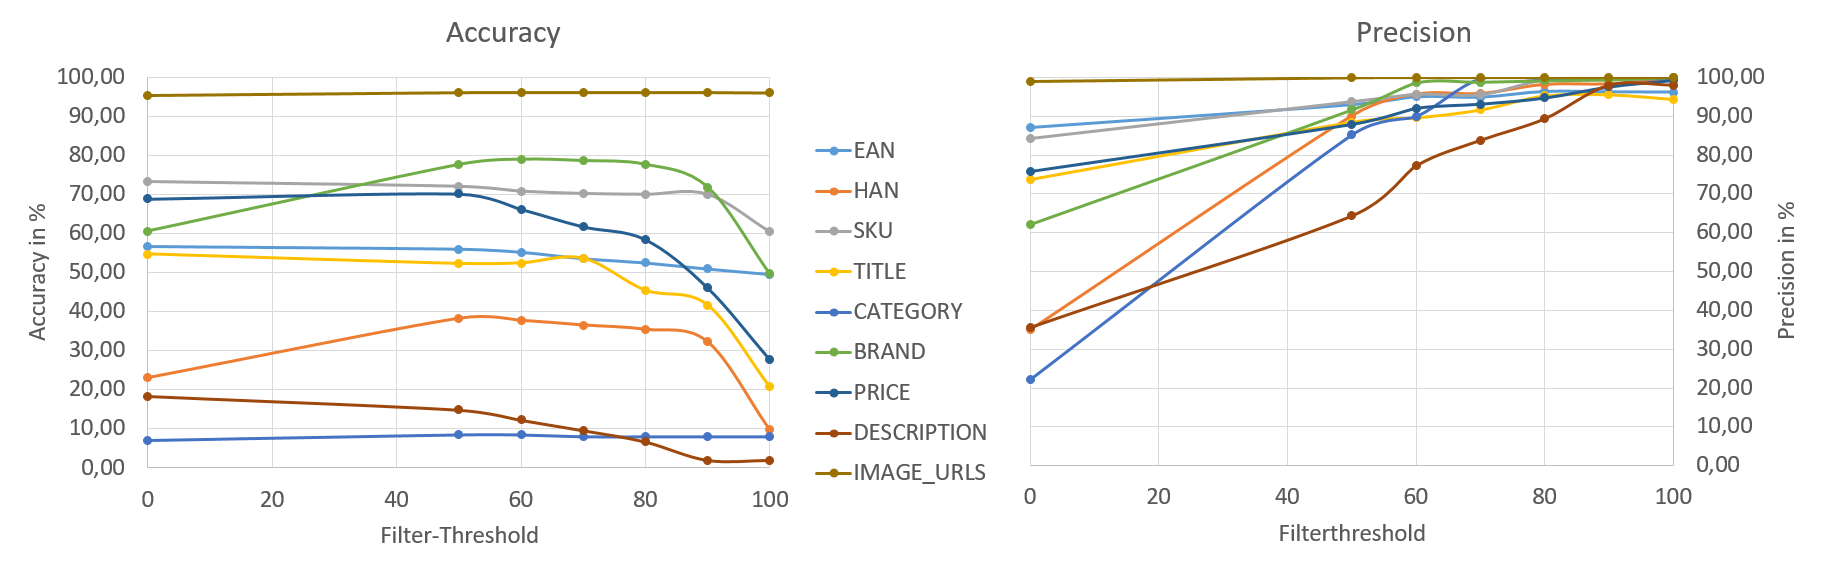
\includegraphics[width=\textwidth]{resources/accuracy-and-precision-per-attribute.PNG}
    \caption{Accuracy (links) und Precision (rechts) pro Attribut für $SaS=50$}
    \label{abb:testdaten}
\end{figure}

Zu guter letzt kann man dem Diagramm entnehmen, dass der Filterschwellwert ein gutes Mittel ist, um die Accuracy und
Precision zu beeinflussen und ein höherer SaS-Wert tendenziell besser ist.

\subsection{Mögliche Fehlerquellen der Messungen}
\label{subsec:fehlerquellen}

Bei einer genaueren Analyse der Testdaten musste leider festgestellt werden, dass beim Herunterladen der
Angebotsseiten eines Shops aufgrund einer Captcha-Absicherung keine nutzbaren Webseiten geliefert wurden.
Für diesen Shop konnten folglich keine Regeln erstellt werden, was sich nachteilig auf die Accuracy auswirkt.

Des Weiteren trifft die in Kapitel~\ref{subsec:annahmen} getroffene Annahme, dass die idealo-Daten nicht von denen der
Shops abweichen, nicht zu.
Die Angebotsdaten werden von idealo teilweise manuell oder durch Normalisierungsprozesse manipuliert, was die
Regelerstellung erschweren kann.
Zudem werden möglicherweise korrekt extrahierte Produktattribute fälschlicherweise als inkorrekt markiert.